\setlength{\arrayrulewidth}{.5mm}
\setlength{\tabcolsep}{5pt}
\renewcommand{\arraystretch}{2}

\subsection{Introduzione}
Il team seguirà la metodologia di progetto RUP, in seguito sono specificati il piano di progetto e le
iterazioni che lo compongono.

\subsection{Piano}
Il piano di progetto si suddivide in 4 fasi temporali:
\begin{itemize}
    \item Inception
    \item Elaboration
    \item Construction
    \item Transition
\end{itemize}
Le attività coinvolte sono le seguenti:
\begin{itemize}
    \item Studio di fattibilità
    \item Raccolta dei requisiti
    \item Analisi e progetto
    \item Implementazione
    \item Test
\end{itemize}
Le varie attività si andranno a distribuire sulle fasi temporali, con una distribuzione eterogenea, che
dipende da quanto una particolare attività è significativa in una certa fase.\\
Qui sotto è raffigurato il processo in un grafico descrittivo:

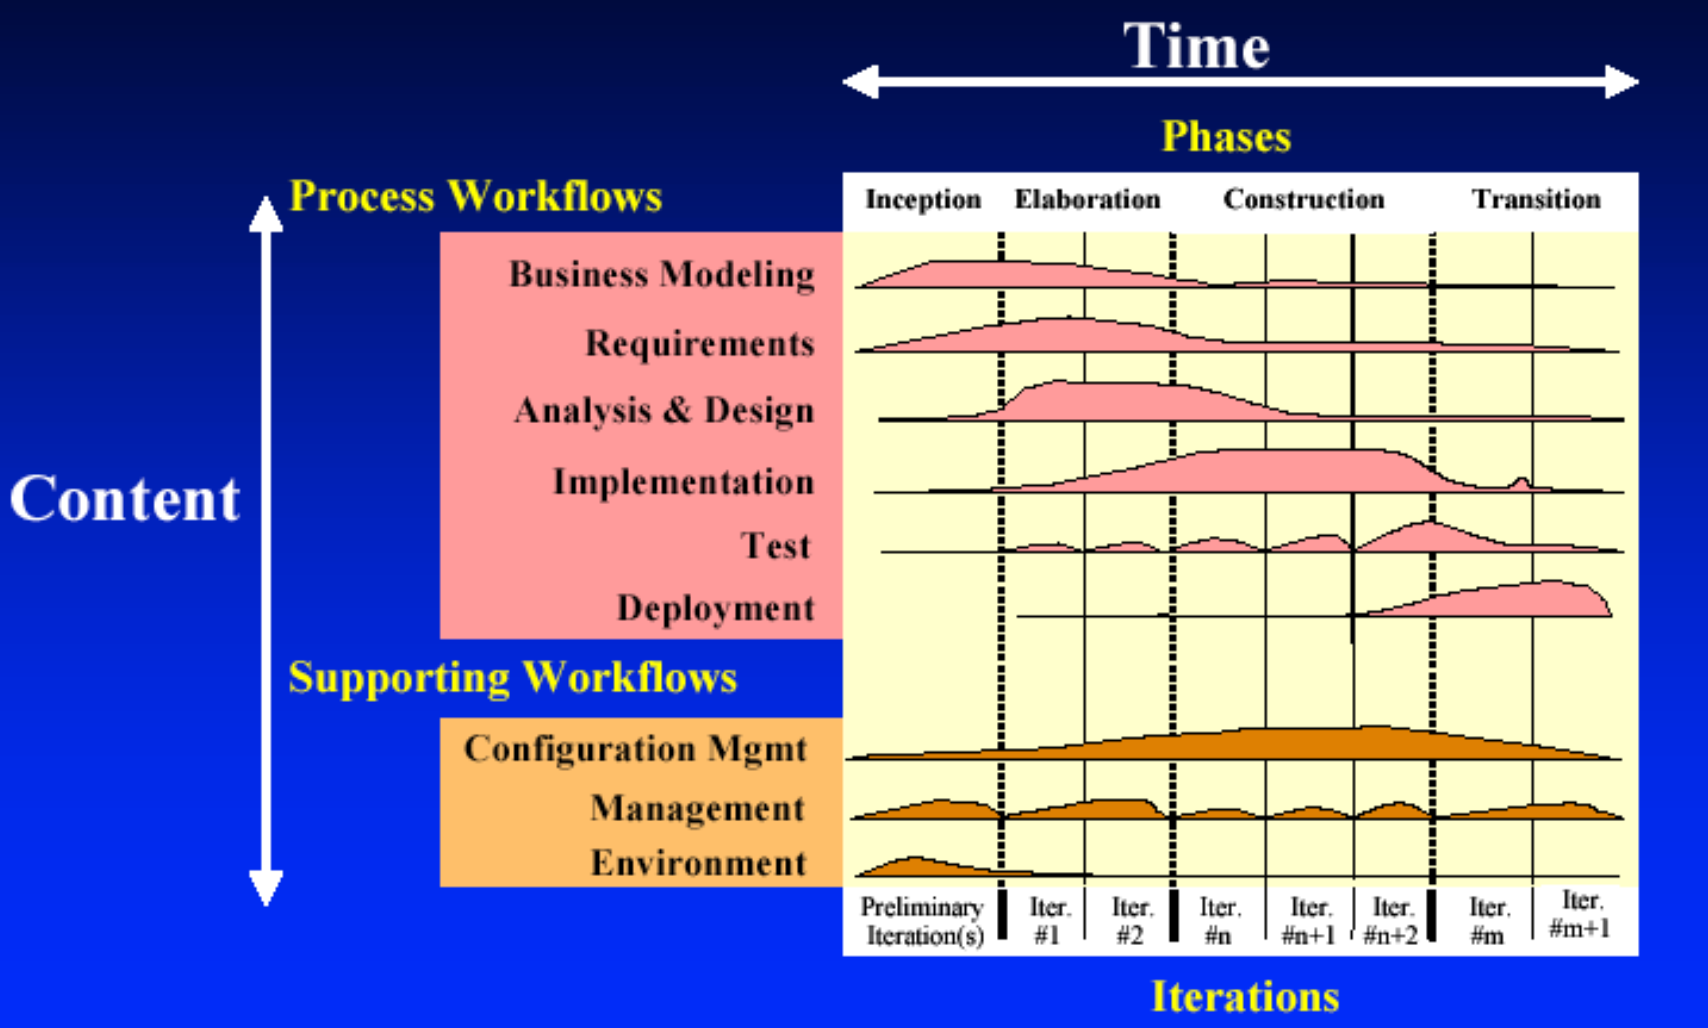
\includegraphics[width=12cm]{images/RUPplan.png}

\subsection{Iterazioni}

\begin{center}

\begin{tabular}{ |p{2cm}|p{10cm}|  }
\hline
Nome & Iterazione 1 \\\hline
Fase & Inception \\\hline
Inizio & 20/11/2019 \\\hline
Fine &  1/12/2019 \\\hline
Obbiettivi & 
	\begin{compactitem}
		\item Analisi del problema e prima stesura del documento di Visione
		\item Proposta configurazione iniziale del sistema
		\item Analisi di fattibilità e stesura del relativo documento
		\item Formulazione prima proposta di Contratto
		\item Formulazione documento Glossario
	\end{compactitem}\\\hline
Stato &  Conclusa \\\hline
\end{tabular}
\label{table:1}\newline

\begin{tabular}{ |p{2cm}|p{10cm}|  }
\hline
Nome & Iterazione 2 \\\hline
Fase & Inception \\\hline
Inizio & 15/12/2019 \\\hline
Fine &  18/12/2019 \\\hline
Obbiettivi & 
	\begin{compactitem}
		\item Raffinamento del documento di Visione
		\item Raffinamento della proposta di Contratto
		\item Stesura del piano di progetto
		\item Aggiornamento del Glossario
	\end{compactitem}\\\hline
Stato &  Conclusa \\\hline
\end{tabular}
\label{table:2}\newline

\begin{tabular}{ |p{1,5cm}|p{10,5cm}|  }
\hline
Nome & Iterazione 3 \\\hline
Fase & Inception \\\hline
Inizio & 19/12/2019 \\\hline
Fine &  31/12/2019 \\\hline
Obbiettivi & 
	\begin{compactitem}
		\item Analisi dei  requisiti e stesura del relativo documento di Specifica
		\item Individuazione dei casi d'uso e assegnamento delle rispettive priorità
		\item Analisi dei Costi e stesura del relativo documento
		\item Analisi e gestione dei rischi e stesura del relativo documento
		\item Aggiornamento del Glossario e del documento di Visione
	\end{compactitem}\\\hline
Stato &  Svolgimento \\\hline
\end{tabular}
\label{table:3}\newline

\begin{tabular}{ |p{2cm}|p{10cm}|  }
\hline
Nome & Milestone 1\\\hline
Fase & Inception \\\hline
Inizio & 1/01/2020 \\\hline
Fine &  1/01/2020 \\\hline
Obbiettivi & 
	\begin{compactitem}
		\item I requisiti principali sono stati individuati e descritti correttamente
		\item Tutti i i rischi sono stati individuati
		\item \'E stata effettuata una stima dei costi fedele
		\item Tutte le iterazioni sono state programmate
	\end{compactitem}\\\hline
Stato &  Programmata \\\hline
\end{tabular}
\label{table:milestone1}\newline

\begin{tabular}{ |p{2cm}|p{10cm}|  }
\hline
Nome & Iterazione 4 \\\hline
Fase & Elaboration \\\hline
Inizio & 2/01/2020 \\\hline
Fine &  18/01/2020  \\\hline
Obbiettivi & 
	\begin{compactitem}
		\item Raffinamento dei documenti Glossario, Requisiti
		\item Definire un modello tabellare dettagliato dei vari casi d'uso
		\item Definire i diagrammi UML dei vari casi d'uso
		\item Creazione di una matrice di tracciabilità
	\end{compactitem}\\\hline
Stato &  Programmata \\\hline
\end{tabular}
\label{table:4}\newline

\begin{tabular}{ |p{2cm}|p{10cm}|  }
\hline
Nome & Iterazione 5 \\\hline
Fase & Elaboration \\\hline
Inizio & 19/01/2020 \\\hline
Fine &  31/01/2020  \\\hline
Obbiettivi & 
	\begin{compactitem}
		\item Creazione schede CRC
		\item Creazione diagramma EBC
		\item Creazione diagrammi di sequenza
		\item Creazione diagrammi di classi
		%\item Definire un coordinamento dei vari casi s'uso
	\end{compactitem}\\\hline
Stato &  Programmata \\\hline
\end{tabular}
\label{table:5}\newline

\begin{tabular}{ |p{2cm}|p{10cm}|  }
\hline
Nome & Iterazione 6 \\\hline
Fase & Elaboration \\\hline
Inizio & 1/02/2020 \\\hline
Fine & 7/02/2020 \\\hline
Obbiettivi & 
	\begin{compactitem}
		\item Raffinamento e revisione dei vari diagrammi definiti durante l'iterazione 5
		\item Realizzazione dei test
	\end{compactitem}\\\hline
Stato &  Programmata \\\hline
\end{tabular}
\label{table:6}\newline

\begin{tabular}{ |p{2cm}|p{10cm}|  }
\hline
Nome & Milestone 2\\\hline
Fase & Elaboration \\\hline
Inizio & 8/02/2020 \\\hline
Fine &  8/02/2020 \\\hline
Obbiettivi & 
	\begin{compactitem}
		\item Devono essere stati definiti correttamente i diagrammi di Sequenza, di classi, UML di casi d'uso, EBC, schede CRC.
	\end{compactitem}\\\hline
Stato &  Programmata \\\hline
\end{tabular}
\label{table:milestone2}\newline

\begin{tabular}{ |p{2cm}|p{10cm}|  }
\hline
Nome & Iterazione 7 \\\hline
Fase & Construction \\\hline
Inizio & 9/02/2020 \\\hline
Fine &  13/02/2020  \\\hline
Obbiettivi & 
	\begin{compactitem}
		\item Creazione di un diagramma architetturale dell'intero sistema
		\item Raffinamento dei test
	\end{compactitem}\\\hline
Stato &  Programmata \\\hline
\end{tabular}
\label{table:7}\newline

\begin{tabular}{ |p{2cm}|p{10cm}|  }
\hline
Nome & Milestone 3\\\hline
Fase & Construction \\\hline
Inizio & 14/02/2020 \\\hline
Fine &  14/02/2020 \\\hline
Obbiettivi & 
	\begin{compactitem}
		\item Il sistema rispetta tutti i requisiti definiti nella fase di analisi
		\item Il sistema ha superato tutti i test definiti in precedenza
	\end{compactitem}\\\hline
Stato &  Programmata \\\hline
\end{tabular}
\label{table:milestone3}\newline

\begin{tabular}{ |p{2cm}|p{10cm}|  }
\hline
Nome & Iterazione 8 \\\hline
Fase & Transition \\\hline
Inizio & 15/02/2020 \\\hline
Fine &  19/02/2020  \\\hline
Obbiettivi & 
	\begin{compactitem}
		\item Raccolta Feedback di utilizzo degli utenti
		\item Revisione generale del sistema
		\item Creare una release finale
	\end{compactitem}\\\hline
Stato &  Programmata \\\hline
\end{tabular}
\label{table:8}\newline

%AGGIUNGERE GANT QUI

\end{center}